\subsection{JSON-Schema}\label{subsec:schema}
Wie im vorherigen Kapitel bereits erwähnt bedient sich die Beschreibung eines Workflows grundlegend der Syntax von~\ac{YAML}.
In Kapitel~\ref{subsubsec:json-schema} wurden bereits die Grundlagen für JSON-Schemas geschaffen, in diesem Kapitel wird das erstellte
fulibWorkflows-Schema genauer betrachtet.
Das Schema ist komplett im Anhang hinterlegt, da dieses zu lang ist, um es übersichtlich in diesem Kapitel zu erläutern.
Dadurch wird nur auf die wichtigsten Punkte der Implementierung eingegangen.
Um die Lesbarkeit für Entwickler zu verbessern, ist das Schema in zwei Dateien aufgeteilt.

\begin{listing}[!ht]
    \inputminted[xleftmargin=20pt,linenos]{json}{listings/3.1.2/page.json}
    \caption{Referenzieren eines anderen Schemas}
    \label{listing:schema-split}
\end{listing}

Listing~\ref{listing:schema-split} ist eine minimale Version des eigentlichen Schemas, in welchem dennoch die wichtigsten Funktionen dargestellt sind.
Das fulibWorkflows-Schema ist in zwei Hauptteile unterteilbar, in die Definitionen und die Festlegung der erlaubten Elemente in der obersten Liste.
Durch das Schema werden nur JSON-/YAML-Dateien akzeptiert, welche aus einer Liste an Elementen bestehen.
Hierbei sind die Elemente jedoch festgelegt durch die in Zeile 20 und 21 dargestellten Zeilen.
Ein \textit{item} darf nur aus einem der Elemente bestehen, welche in der Auflistung ab Zeile 22 festgelegt sind.
Um die Lesbarkeit zu vereinfachen und die Schachtelungstiefe möglichst gering zu halten, werden die erlaubten Elemente lediglich referenziert.
Die referenzierten Elemente wurden im ersten Teil des Schemas, ab Zeile 4, definiert.
Für jedes der im vorherigen Kapitel erwähnten Zettel, gibt es ein Element im Schema.
Die Definitionen der Elemente, welche nicht in Listing~\ref{listing:schema-split} dargestellt sind, enthalten lediglich Standardwerte, welche bereits in Kapitel~\ref{subsubsec:json-schema} erläutert wurden.
Diese können im Anhang nachgelesen werden.
Die Definition der Page ist jedoch ein Sonderfall, welche durch das Aufteilen in mehrere Dateien entstanden ist.
Es ist möglich weitere Schemas aus einer anderen Datei zu importieren, dies ist in Zeile 11 ersichtlich.
Auch dort wird erneut ein Referenzieren durchgeführt, allerdings nicht auf eine im Schema befindlichen Definition, sondern auf die Page Definition aus der \textit{page.schema.json} Datei.
Die Aufteilung wurde durchgeführt, da die Page eine Liste ist und ebenfalls fünf eigene Elemente definiert.
Allein das Page-Schema beläuft sich auch 93 Zeilen und umfasst somit allein die Hälfte des Parent-Schemas.

Wie in Kapitel~\ref{subsubsec:json-schema} bereits erwähnt, ist das fulibWorkflows-Schema ebenfalls bei Schemastore.org hinterlegt.
Es wird automatisch für Dateien mit der Dateiendung \textit{.es.yaml} vom Editor verwendet.
Dadurch ist es zum Beispiel in IntelliJ möglich Autovervollständigung für fulibWorkflows zu bekommen und auf Fehler hingewiesen zu werden.

\begin{figure}%
    \centering
    \subfloat[\centering Leere Datei]{{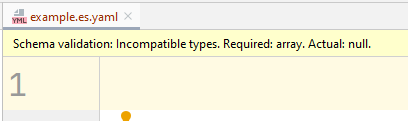
\includegraphics[width=6cm]{images/3.1/Empty} }}%
    \qquad
    \subfloat[\centering Fehlerhafte Eingabe]{{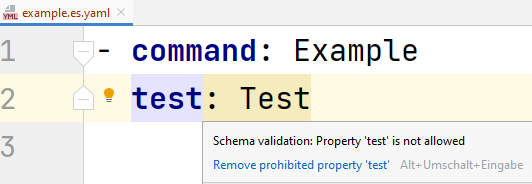
\includegraphics[width=7cm]{images/3.1/fails} }}%
    \caption{Fehleranzeige in IntelliJ}%
    \label{fig:errors-schema}%
\end{figure}

In Abbildung~\ref{fig:errors-schema} ist das Hervorheben von Fehlern in IntelliJ dargestellt, welches durch das JSON-Schema generiert wird.
In Abbildung~\ref{fig:errors-schema}((a)) ist die Datei leer, wodurch die Schema Validierung anschlägt und den Entwickelnden darauf hinweist, dass ein Array, also eine Liste an Elementen, benötigt wird.
Sobald ein Element begonnen wird, wird diese Warnung nicht mehr angezeigt.
Sollte der Entwickelnde wiederum ein Element hinzufügen, welches keinem der definierten Elemente des Schemas entspricht, wird die Meldung aus Abbildung~\ref{fig:errors-schema}((b)) angezeigt.
Da ein Command keine zusätzlichen Attribute/Properties akzeptiert, dennoch eines hinzugefügt wurde, besagt der Fehler, dass es nicht erlaubt ist weitere Attribute hinzuzufügen.

\begin{figure}%
    \centering
    \subfloat[\centering Alle Elemente]{{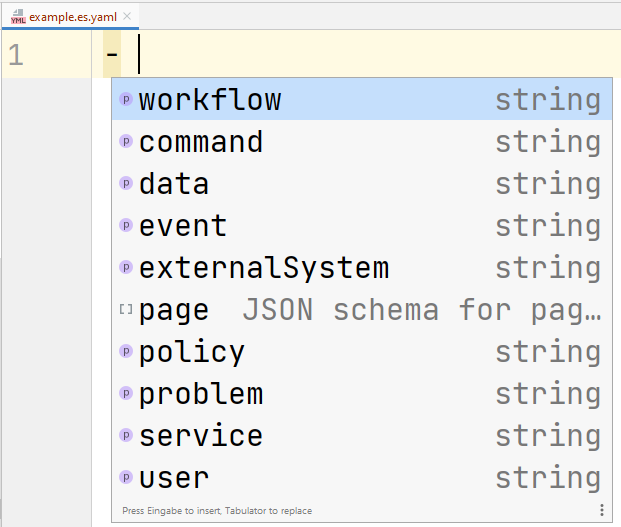
\includegraphics[width=6cm]{images/3.1/all} }}%
    \qquad
    \subfloat[\centering Page Elemente]{{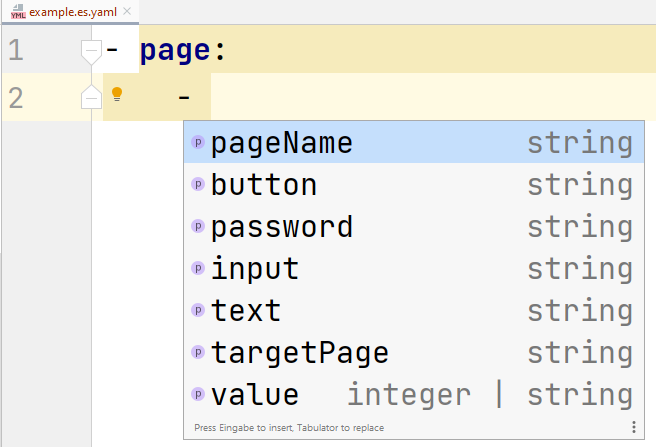
\includegraphics[width=6cm]{images/3.1/page} }}%
    \caption{Autovervollständigung in IntelliJ}%
    \label{fig:completion-schema}%
\end{figure}

Wie zuvor erwähnt ermöglicht ein Schema jedoch nicht nur das Hervorheben von Fehlern, sondern unterstützt den Entwickelnden zusätzlich durch Autovervollständigung.
Dies ist in Abbildung~\ref{fig:completion-schema} dargestellt.
Hierbei wird aufgrund des Kontextes verschiedene Möglichkeiten von zu erstellenden Elementen vorgeschlagen.
Auf oberster Ebene werden alle erlaubten Schlüsselwörter für Elemente angezeigt, welches in Abbildung~\ref{fig:completion-schema}((a)) dargestellt ist.
Hierbei fällt auf, dass die Elemente für eine Page nicht angezeigt werden, dies ist jedoch der Fall, sobald der Kontext dies zulässt.
Während der Entwickelnde ein page-Element definiert, werden wie in Abbildung~\ref{fig:completion-schema}((b)) dargestellt die Schlüsselwörter für Page-Elemente vorgeschlagen.
